\begin{refsection}[research/miyoshi/group.bib]
\nocite{*}
\chapter{Data Assimilation Research Team}

\section{Members}

\begin{itemize}
\item[] Takemasa Miyoshi (Team Leader)
\item[] Koji Terasaki (Research Scientist)
\item[] Shigenori Otsuka (Postdoctoral Researcher)
\item[] Keiichi Kondo (Postdoctoral Researcher)
\item[] Shunji Kotsuki (Postdoctoral Researcher)
\item[] Guo-Yuan Lien (Postdoctoral Researcher)
\item[] Takumi Honda (Postdoctoral Researcher)
\item[] Yasumitsu Maejima (Research Associate)
\item[] Africa Perianez Santiago (Research Associate)
\item[] Hazuki Arakida (Technical Staff)
\item[] Gulanbaier Tuerhong (Technical Staff)
\item[] Juan J. Ruiz (Visiting Scientist)
\item[] Shinichiro Shima (Visiting Scientist)
\item[] Shu-Chih Yang (Visiting Scientist)
\item[] Stephen G. Penny (Visiting Scientist)
\item[] Masaru Kunii (Visiting Scientist)
\item[] Kozo Okamoto (Visiting Scientist)
\item[] Michiko Otsuka (Visiting Scientist)
\item[] Marimo Ohhigashi (Research Assistant)
\item[] Yaping Chang (International Program Associate)
\item[] Yukie Komori (Assistant)
\item[] Rie Deguchi (Assistant)
\end{itemize}

\section{Research Activities}

The Data Assimilation Research Team (DA Team) was launched in October 2012 and is composed of 18 research and technical staff including 7 visiting members as of March 2016. Data assimilation (DA) is a cross-disciplinary science to synergize computer simulations and real-world data, based on statistical mathematics and dynamical systems theory. As computers advance and enable precise simulations, it will become more important to compare the simulations with real-world data. DA Team performs cutting-edge research and development on advanced DA methods and their wide applications, aiming to integrate computer simulations and real-world data in the wisest way. Particularly, DA Team tackles challenging problems of developing efficient and accurate DA systems for ``big simulations'' with real-world ``big data'' from various sources including advanced sensors. The specific foci include 1) theoretical and algorithmic developments for efficient and accurate DA, 2) DA methods and applications by taking advantage of the world-leading K computer and ``big data'' from new advanced sensors, and 3) exploratory new applications of DA in wider simulation fields. These advanced DA studies will enhance simulation capabilities and lead to a better use of high-performance computers including the leading-edge K computer.

In FY2015, we continued on the ongoing data assimilation research in the following aspects: 1) theoretical research on challenging problems, 2) leading research on meteorological applications, 3) optimization of computational algorithms, and 4) exploratory research on wider applications. We also continued close collaborations with several research teams within the AICS Research Division. We have made substantial progress on the following research items:


\paragraph{Theoretical research}
\begin{itemize}
  \setlength{\parskip}{0cm}
  \setlength{\itemsep}{0cm}

\item A paper on the discrete Bayesian optimization approach to find optimal ensemble sizes in a multi-model ensemble Kalman filter (EnKF) was published (1 paper published).

\item A new local particle filter method to treat non-Gaussian PDF was explored (1 paper submitted).
\end{itemize}

\paragraph{Leading research on meteorological applications}
\begin{itemize}
  \setlength{\parskip}{0cm}
  \setlength{\itemsep}{0cm}

\item We have successfully run the largest-ever ensemble DA experiments with 10,240 samples for the global atmosphere using real observations with the real-case Nonhydrostatic ICosahedral Atmospheric Model (NICAM) (1 paper published, press release on November 11, 2015).

\item Impact of localization in ensemble Kalman filter was investigated with 10,240 samples using an intermediate AGCM (1 paper submitted).

\item Non-Gaussian statistics in the global atmospheric dynamics were investigated with the 10,240-sample ensemble Kalman filter using an intermediate AGCM.

\item Multi-scale data assimilation was investigated based on 10,240-member ensemble Kalman filter using an intermediate AGCM and NICAM.

\item A DA system for Advanced Microwave Sounding Unit (AMSU)-A radiance data was developed with NICAM-LETKF.

\item A DA system for JAXA's Global Satellite Mapping of Precipitation (GSMaP) data was developed with NICAM-LETKF.

\item A high resolution experiment using NICAM-LETKF system assimilating the conventional, AMSU-A, and GSMaP observations has been performed on the K computer.

\item The spatial and inter-channel observation error correlations of AMSU-A were investigated with the NICAM-LETKF system.

\item An earlier study on the assimilation of global precipitation data with the low-resolution NCEP GFS model were summarized and published (2 papers published).

\item A paper on the new quality control algorithm for the Osaka Phased Array Weather Radar (PAWR) was published (1 paper published).

\item The LETKF system with the SCALE model (SCALE-LETKF) was developed and improved in collaboration with Computational Climate Science Research Team. Several new functions,
  including PAWR assimilation, Himawari-8 satellite data assimilation,
  relaxation-to-prior-spread (RTPS) method, offline-nested domains, were implemented with the SCALE-LETKF system.

\item A near-real-time regional weather analysis and forecast system based on the SCALE-LETKF has been set up and run on the K computer.
  It has produced weather analyses and 5-day forecasts every 6 hours for more than 9 months.

\item The ``Big Data Assimilation'' experiments for a local severe rainstorm case were performed with the SCALE-LETKF system, assimilating the PAWR data.
  The results were compared with the previous NHM-LETKF experiments and the nowcasting experiments (1 paper submitted).

\item A project-wide paper for ``Big Data Assimilation'' with the first results of NHM-LETKF experiments was accepted for publication (1 paper accepted).

\item Model output statistics have been investigated using machine learning algorithms and deep learning algorithms.

\item Convective predictability was investigated by performing breeding experiments. Dependency on the model resolution was investigated.

\item A precipitation nowcasting system was developed to take advantage of the dense and frequent PAWR data (1 paper published).

\item A space-time extrapolation system for GSMaP with DA was developed using LETKF.
  The system has been running in real time since January 2016 (1 paper accepted in June 2016).

\item A new Himawari-8 observation operator for SCALE-LETKF was developed and tested with a tropical cyclone case.

\item Himawari-8 may capture clouds at an earlier stage of convective development before a radar captures large raindrops. This potential advantage was explored.

\item The potential usage of Himawari-8 observation for estimating microphysics parameters through DA was explored.

\item A 4-dimensional NHM-LETKF system was developed to investigate a fail-safe workflow and the relationship between the DA window length and forecast accuracy.

\item A series of DA experiments for a sudden local severe rainstorm case in Kobe on September 11, 2014 was performed to investigate the predictability.
\end{itemize}

\paragraph{Computational optimization}

\begin{itemize}
  \setlength{\parskip}{0cm}
  \setlength{\itemsep}{0cm}

\item Huge-jobs, computing the ``Big Data Assimilation'' problem with the SCALE-LETKF, as big as near full nodes of the K computer were performed to measure the computational time and scalability of the code.

%\item Large ensemble

%\item The computational performance of NICAM-LETKF was improved in collaboration with the Computational Climate Science Research Team (1 paper published).
\end{itemize}

\paragraph{Wider applications}

\begin{itemize}
  \setlength{\parskip}{0cm}
  \setlength{\itemsep}{0cm}

\item A particle filter was applied to a dynamical vegetation model known as the SEIB-DGVM (Spatially-Explicit, Individual-Based Dynamic Global Vegetation Model).
  Uncertainties in the state variables and the parameters were greatly reduced by assimilating satellite based Leaf Area Index.

\item Land surface DA system was developed with SiBUC (Simple Biosphere including Urban Canopy) model and LETKF.

\item A global crop calendar was estimated with the satellite-sensed vegetation index (1 paper published).

\item Impacts of satellite-based solar radiation data on land surface simulations were estimated (1 paper published).
\end{itemize}

Several achievements are selected and highlighted in the next section.

\section{Research Results and Achievements}


\subsection{Big Ensemble Data Assimilation in Numerical Weather Prediction}
\locallabel{sec:big_ensemble_da}
Taking advantage of the K computer,
we have successfully run the largest-ever ensemble DA experiments with 10,240 samples for the global atmosphere
with the real-case Nonhydrostatic ICosahedral Atmospheric Model (NICAM) (Miyoshi et al. 2015)
using the NICAM-LETKF (Local Ensemble Transform Kalman Filter) system developed in FY2014 (Terasaki et al. 2015).
This research result was highlighted by RIKEN Press Release on November 11, 2015.
The samples size of 10,240 is two orders of magnitude larger than the typical choice of about 100. The computational cost for the ensemble DA is proportional to the cubic power of the sample size, and active collaborations with AICS Large-scale Parallel Numerical Computing Technology Research Team (PI: Dr. T. Imamura) played an essential role in accelerating the computation by a factor of 8 using an eigenvalue solver “EigenExa” optimized for the K computer. The large sample size reduces the sampling error (Fig. \localref{fig:1}), and we discovered potential long-range correlations up to about 7,000 km (Fig. \localref{fig:1} b). This suggests potential use of faraway observations to improve numerical weather prediction (NWP), although we usually assume that the impact of observations is limited within a range up to 4,000 km or so. The large ensemble DA experiments would provide fundamental datasets to improve our knowledge on the flow-dependent error statistics including non-Gaussian and multi-scale structures, and would help develop advanced approaches for non-Gaussian and multi-scale DA, the topics at the center of theoretical DA research.

\begin{figure}
\centering
  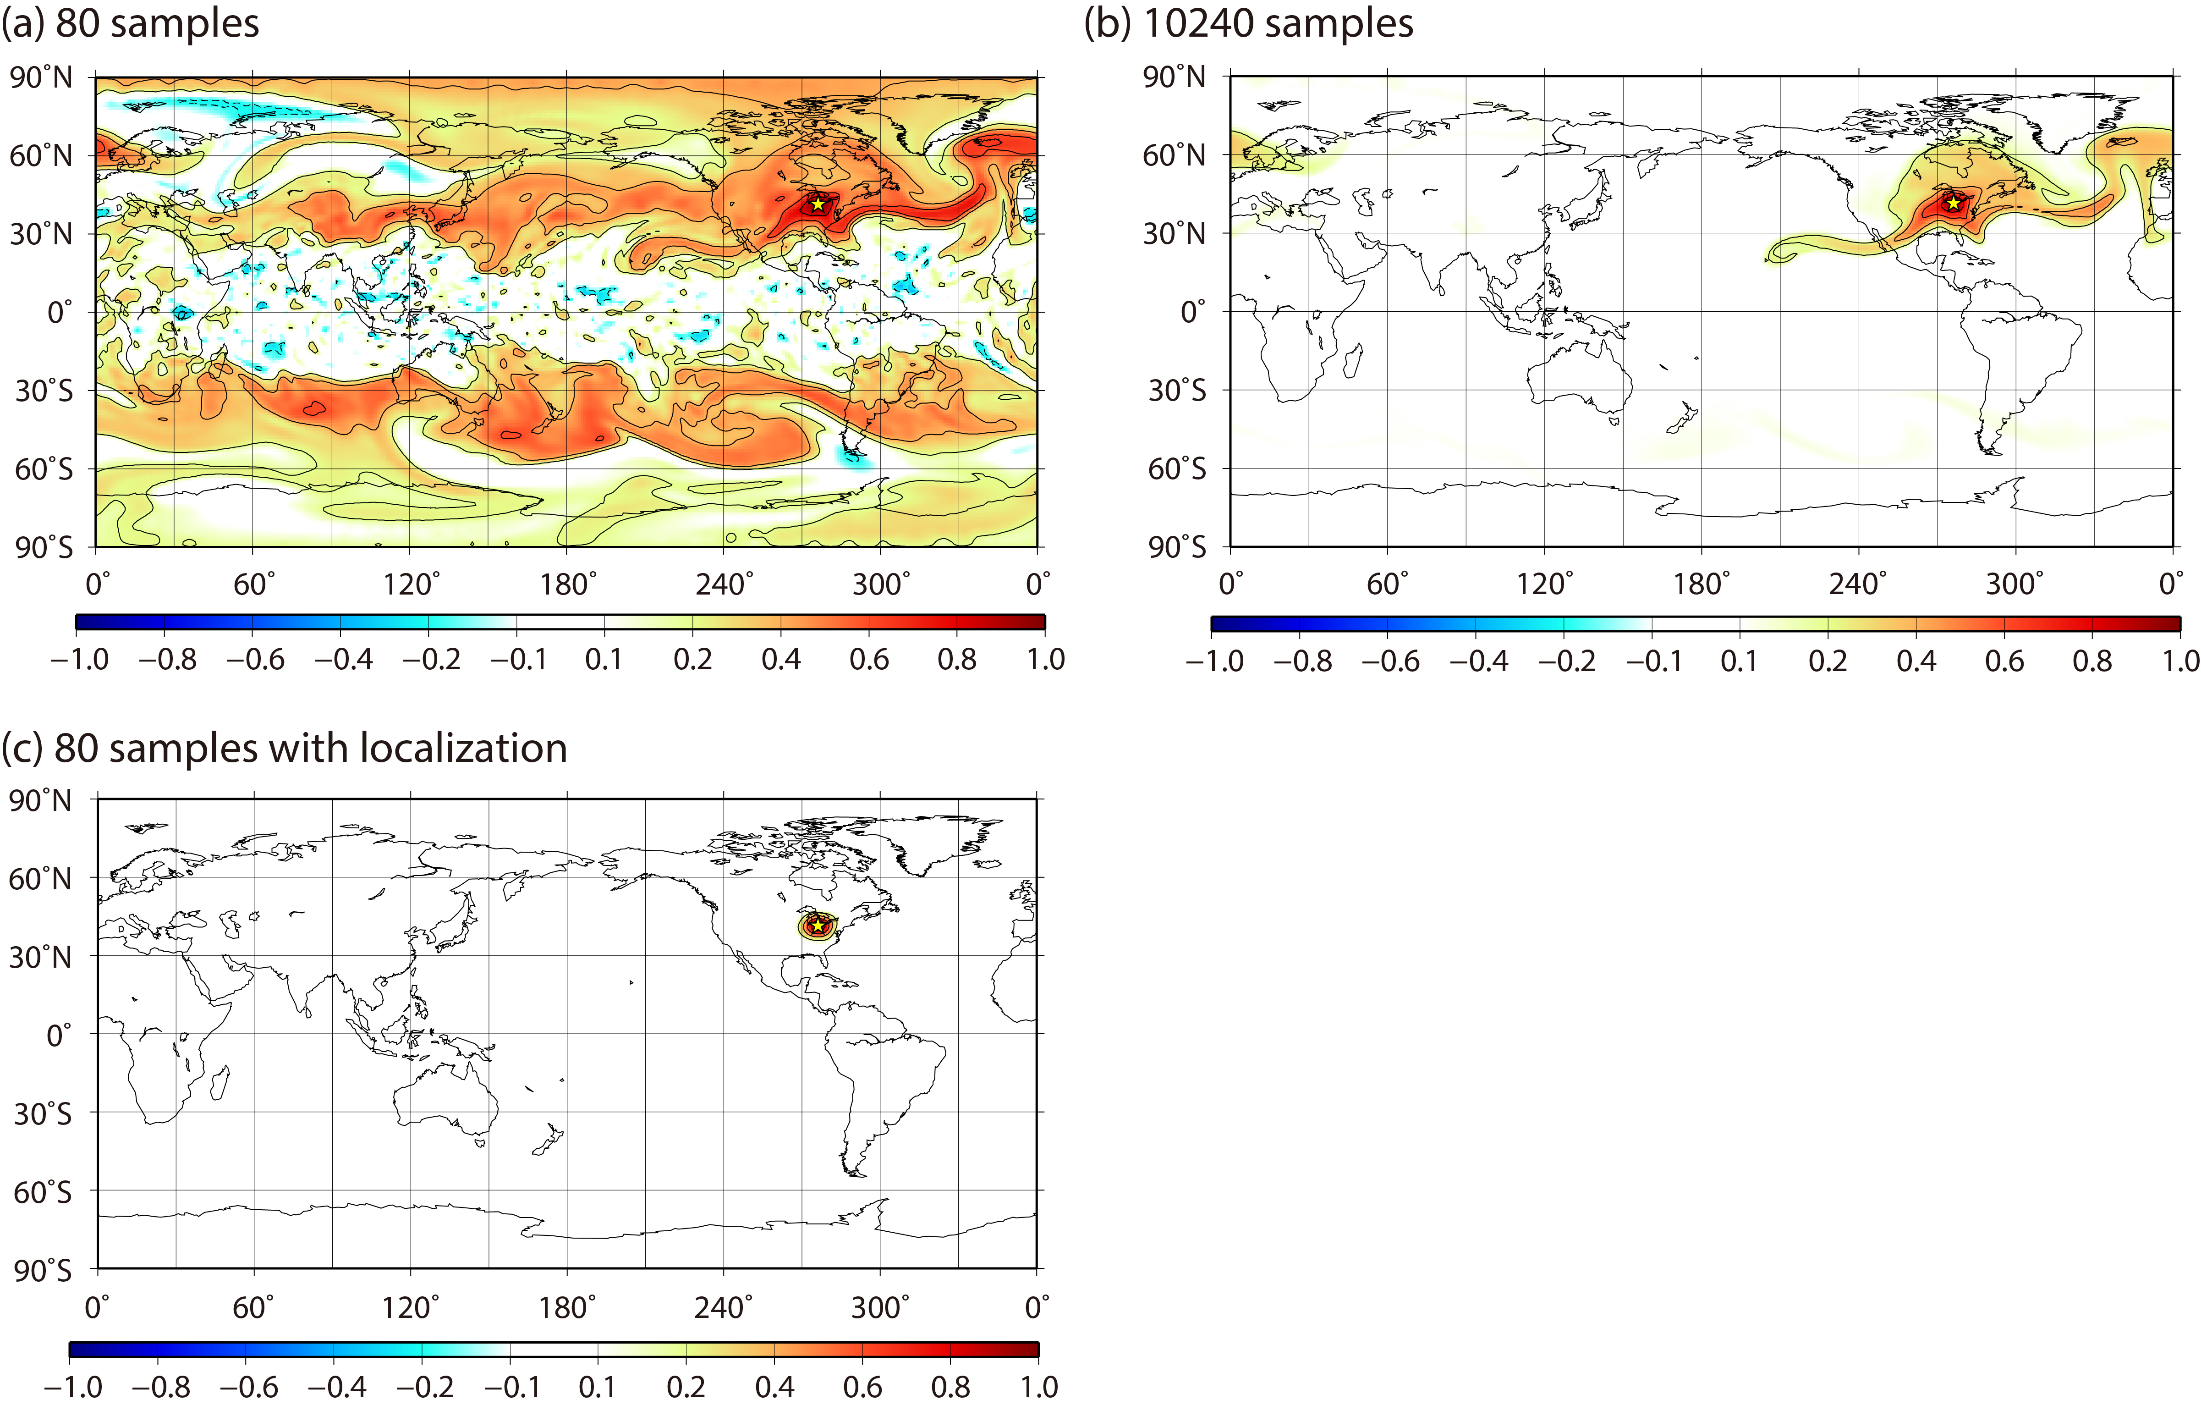
\includegraphics[width=0.99\textwidth,keepaspectratio,natwidth=193,natheight=40,clip,trim=0 240 0 0]
  {research/miyoshi/miyoshi-team-fig1.png}
  \caption{Horizontal maps of real atmosphere autocorrelations with (a) 80 samples and (b) 10240 samples. Adopted from Fig. 5 of Miyoshi et al. (2015), \copyright IEEE 2015.}
  \locallabel{fig:1}
\end{figure}

\subsection{Near-real-time Implementation of Regional Numerical Weather Prediction (NWP)}
The LETKF-based DA system has been newly developed with the regional NWP model ``SCALE'' in collaboration with Computational Climate Science Research Team (PI: Dr. H. Tomita). Real-world observation data are available from the US National Centers for Environmental Prediction (NCEP) in near real time, by about 3-hour delay from the real time. We have implemented the near-real-time 5-day NWP using the SCALE-LETKF system, and have been running continuously from May 7, 2015. Figure \localref{fig:3} indicates an example of a forecast in a case of the worst disaster in 2015 by flooding of River Kinugawa, Tochigi, Japan. The line-type system is well simulated. By continuously running SCALE-LETKF analysis and forecasts, we accumulate experiences and verification samples, which will be very useful for further improvements of DA and NWP system developments.

\begin{figure}
\centering
  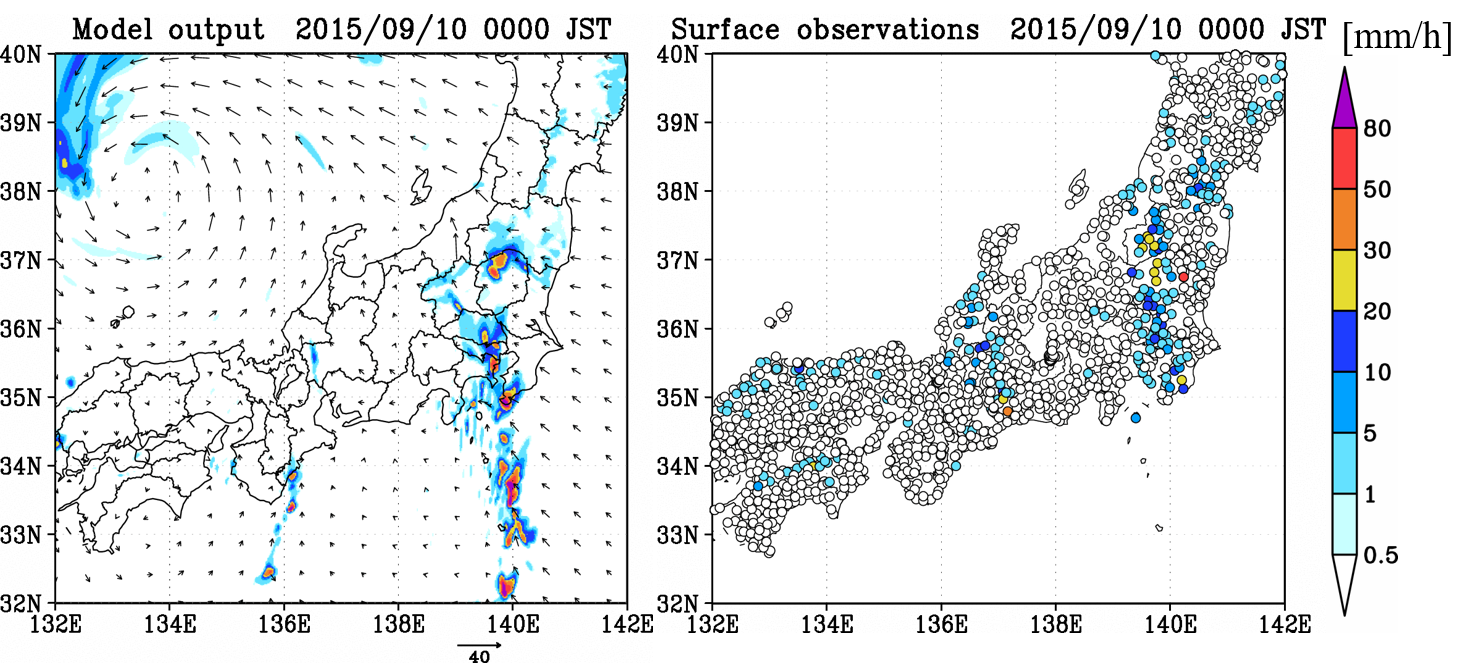
\includegraphics[width=0.99\textwidth,keepaspectratio,natwidth=193,natheight=40]
  {research/miyoshi/miyoshi-team-fig3.png}
  \caption{1-hour accumulated rainfall amount at 0000 JST, September 10, 2015, when River Kinugawa had flooded and caused severe disasters, from a model simulation initiated at 1200 JST, September 8 (left) and surface rain-gauge observation (right) from NTT Docomo environmental sensor network.}
  \locallabel{fig:3}
\end{figure}

\subsection{Effective Use of Satellite Big Data}
Developing DA methods for effective use of various observation data is important. Satellite remote sensing provides a relatively uniform coverage of a broad area of the globe, and plays an essential role in NWP. However, the observed quantities are not direct to the prognostic variables of NWP models, and the data volume and variety keep increasing rapidly as sensor technology advances. Therefore, satellite DA requires algorithmic and methodological developments, and has become a major field in meteorology. We have been actively working on the research on effective assimilation of satellite-based precipitation data including the GPM (global precipitation measuring mission) core satellite data in collaboration with JAXA (Japan Aerospace Exploration Agency), microwave radiances from low-earth orbit satellites, and big data from the new-generation geostationary satellite Himawari-8 in collaboration with JMA (Japan Meteorological Agency) Meteorological Satellite Center and Meteorological Research Institute. Figure \localref{fig:4} shows an example of the impact of assimilating Himawari-8 infrared radiances in the case of Typhoon Soudelor 2015. The outer rainbands north of the vortex are greatly enhanced by assimilating Himawari-8 and becomes much closer to the observation.


\begin{figure}
\centering
  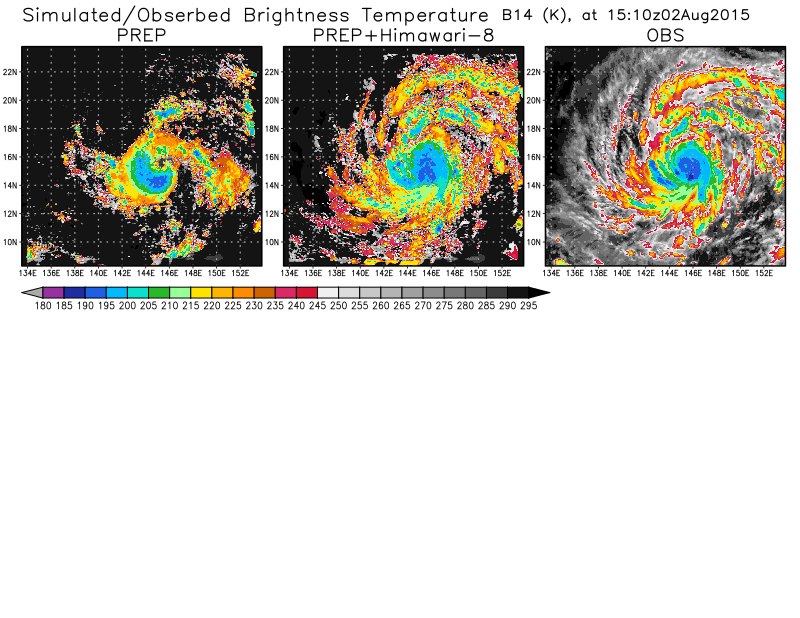
\includegraphics[width=0.99\textwidth,keepaspectratio,natwidth=193,natheight=40,clip,trim=0 230 0 0]
  {research/miyoshi/miyoshi-team-fig4.png}
  \caption{Geostationary satellite Himawari-8 band-14 brightness temperature (K) at 1510 UTC, August 2, 2015 (right) and simulated images with/without assimilating Himawari-8 data (center/left).}
  \locallabel{fig:4}
\end{figure}

\subsection{New Application with Individual-based Dynamical Vegetation Model}
As a new explorative application of DA, we have been working on land-surface and vegetation applications. We have successfully applied DA to the Spatially-Explicit Individual-Based Dynamic Global Vegetation Model (SEIB-DGVM) for the first time. The individual-based model simulates individual plants explicitly; some trees may die, while new trees may emerge. Therefore, the model prognostic variables such as tree height and root depth may change time to time and place to place. Typical DA methods assume the phase space to be predefined and never change. Alternatively, we applied a SIR (Sequential Importance Resampling) particle filter. The results were encouraging. Figure \localref{fig:5} shows the results with the real satellite-based MODIS (Moderate Resolution Imaging Spectroradiometer) LAI (Leaf Area Index) observations at a single location. It is not surprising that the uncertainties of the simulated LAI are reduced significantly (Fig. \localref{fig:5} a), but we also find that the uncertainties of unobserved model parameters and variables are reduced significantly (Fig. \localref{fig:5} b, c).

\begin{figure}
\centering
  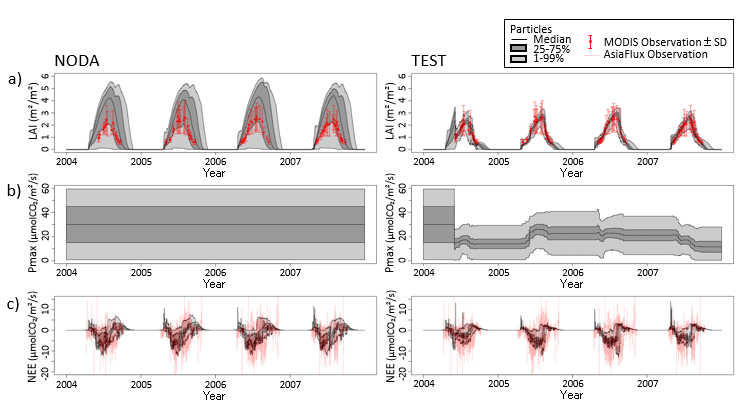
\includegraphics[width=0.99\textwidth,keepaspectratio,natwidth=193,natheight=40]
  {research/miyoshi/miyoshi-team-fig5.png}
  \caption{4-year time series of (a) LAI, (b) a model parameter (maximum photosynthesis rate), and (c) a model variable (net ecosystem exchange) for the cases without DA (left) and with DA (right). Adopted from Arakida et al. (2016, \textit{Nonlin.\ Processes Geophys.\ Discuss.}).}
  \locallabel{fig:5}
\end{figure}

\subsection{Theoretical and algorithmic developments}
\locallabel{sec:theoretical}
Theoretical DA research is an important part of DA Team’s scope. Here, we highlight some of the major theoretical developments in FY2015.
A paper on the discrete Bayesian optimization approach to find optimal ensemble sizes in a multi-model ensemble Kalman filter (EnKF) was published (Otsuka and Miyoshi 2015).
Potential impact of assimilation order of observations in serial EnKF was investigated (Kotsuki et al., manuscript in preparation).
A new local particle filter method to treat non-Gaussian PDF was explored (Penny and Miyoshi 2016, \textit{Nonlin.\ Processes Geophys.\ Discuss.}).


%Text for research Results and achievements. Journal-artcile~\cite{sample-journal}.
%Conference-paper~\cite{sample-conference}.
%Invited-talk~\cite{sample-invited}.
%For cross referencing, use \verb|\locallabel| and \verb|\localref| to avoid conflicting names defined by other groups. For example, a figure can be referenced as Figure~\localref{fig:sample-label1}.

%\begin{figure}
%\centering
%  \includegraphics[width=0.5\textwidth,keepaspectratio,natwidth=193,natheight=40]
%  {sample_division/sample_group/test1.png}
%  \caption{Caption for a sample figure}
%  \locallabel{fig:sample-label1}
%\end{figure}

\section{Schedule and Future Plan}

In FY2015, DA team had one additional full-time research staff, and the team will grow further in FY2016.
DA team has been exploring various aspects of DA including theoretical problems, meteorological applications, and wider applications,
with large-scale computing to fully utilize ``Big Data.''
We have very strong projects in weather forecast applications supported by the JST CREST program, JAXA, and MEXT FLAGSHIP 2020 project.
We will continue our efforts in each topic in FY2016.

``Big Data Assimilation'' (BDA) is one of the major activities that we have developed in FY2015.
The prototype system showed promising results, but the computing speed with the K computer did not meet the requirement for real-time implementation.
Also, the physical performance for the 30-minute forecast of precipitation patterns needs to be improved.
In FY2016, we will continue to work on the development of the BDA system to further improve the computational and physical performances.

In FY2016, we also plan to enhance close collaborations with experts in mathematics, sensor technology, and various application fields.
Enhancing collaborations with other AICS Research Teams will also be beneficial.


\section{Publications}
\section*{Journal Articles}
\begin{enumerate}
  \renewcommand*\labelenumi{[\theenumi]}
\item
  Lien, G.-Y., T. Miyoshi, and E. Kalnay: ``Assimilation of TRMM Multisatellite Precipitation Analysis with a low-resolution NCEP Global Forecast System'', Mon. Wea. Rev., Vol.144, p.643--661, 2016.
\item
  Lien, G.-Y., E. Kalnay, T. Miyoshi, and G. J. Huffman: ``Statistical properties of global precipitation in the NCEP GFS model and TMPA observations for data assimilation'', Mon. Wea. Rev., Vol.144, p.663--379, 2016.
\item
  Otsuka, S., G. Tuerhong, R. Kikuchi, Y. Kitano, Y. Taniguchi, J. J. Ruiz, S. Satoh, T. Ushio, and T. Miyoshi: ``Precipitation nowcasting with three-dimensional space-time extrapolation of dense and frequent phased-array weather radar observations'', Weather and Forecasting, Vol.31, p.329--340, 2016.
\item
  Dillon, M. E., Y. G. Skabar, J. Ruiz, E. Kalnay, E. A. Collini, P. Echevarr\'{i}a, M. Saucedo, T. Miyoshi, and M. Kunii: ``Application of the WRF-LETKF Data Assimilation System over Southern South America: Sensitivity to model physics'', Weather and Forecasting, Vol.31, p.217--236, 2016.
\item
  Hattori, M., J. Matsumoto, S. Ogino, T. Enomoto, and T. Miyoshi: ``The Impact of Additional Radiosonde Observations on the Analysis of Disturbances in the South China Sea during VPREX2010'', SOLA, Vol.12, p.75--79, 2016.
\item
  Sluka, T. C., S. G. Penny, E. Kalnay, and T. Miyoshi: ``Assimilating atmospheric observations into the ocean using strongly coupled ensemble data assimilation'', Geophys. Res. Lett., Vol.43, p.752--759, 2016.
\item
  Sueyoshi T., K. Saito, S. Miyazaki, J. Mori, T. Ise, H. Arakida, R. Suzuki, A. Sato, Y. Iijima, H. Yabuki, H. Ikawa, T. Ohta, A. Kotani, T. Hajima, H. Sato, T. Yamazaki, A. Sugimoto: ``The GRENE-TEA model intercomparison project (GTMIP) Stage 1 forcing data set'', Earth Syst. Sci. Data, Vol.8, p.1--14, 2016.
\item
  Miyoshi, T., M. Kunii, J. Ruiz, G.-Y. Lien, S. Satoh, T. Ushio, K. Bessho, H. Seko, H. Tomita, and Y. Ishikawa: ``"Big Data Assimilation" Revolutionizing Severe Weather Prediction'', Bulletin of the American Meteorological Society, 2016.
\item
  Otsuka, M., M. Kunii, H. Seko, K. Shimoji, M. Hayashi, K. Yamashita: ``Assimilation Experiments of MTSAT Rapid Scan Atmospheric Motion Vectors on a Heavy Rainfall Event'', Journal of the Meteorological Society of Japan. Ser. II, Vol.93, 4, p.459--475, 2015.
\item
  J. Ruiz and M. Pulido: ``Parameter Estimation Using Ensemble Based Data Assimilation in the Presence of Model Error'', Mon. Wea. Rev, Vol.143, p.1568--1582, 2015.
\item
  Seko, H., M. Kunii, S. Yokota, T. Tsuyuki, and T. Miyoshi: ``Ensemble experiments using a nested LETKF system to reproduce intense vortices associated with tornadoes of 6 May 2012 in Japan'', Progress in Earth and Planetary Science, Vol.2:42, 2015.
\item
  Kotsuki S., H. Takenaka, K. Tanaka, A. Higuchi and T. Miyoshi: ``1-km-resolution land surface analysis over Japan: Impact of satellite-derived solar radiation'', Hydrological Research Letters, Vol.9(1), p.14--19, 2015.
\item
  Sawada, M., T. Sakai, T. Iwasaki, H. Seko, K. Saito and T. Miyoshi: ``Assimilating high-resolution winds from a Doppler lidar using an ensemble Kalman filter with lateral boundary adjustment'', Tellus A 2015, Vol.67, p.23473, 2015.
\item
  Chang, C.-C., S.-C. Yang and C. Keppenne: ``Applications of the mean re-recentering scheme to improve typhoon track prediction: A case study of typhoon Nanmadol (2011)'', JMSJ Ser. II, Vol.92, 6, p.559--584, 2015.
\item
  Miyoshi, Takemasa; Kondo, Keiichi; Terasaki, Koji: ``Big Ensemble Data Assimilation in Numerical Weather Prediction'', COMPUTER, Vol.48, p.15--21, 2015.
\item
  Otsuka, Shigenori; Miyoshi, Takemasa: ``A Bayesian Optimization Approach to Multimodel Ensemble Kalman Filter with a Low-Order Model'', MONTHLY WEATHER REVIEW, Vol.143, p.2001--2012, 2015.
\item
  Kotsuki, S.; Tanaka, K.: ``SACRA - a method for the estimation of global high-resolution crop calendars from a satellite-sensed NDVI'', HYDROLOGY AND EARTH SYSTEM SCIENCES, Vol.19, p.4441--4461, 2015.
\item
  Miyazaki, S.; Saito, K.; Mori, J.; Yamazaki, T.; Ise, T.; Arakida, H.; Hajima, T.; Iijima, Y.; Machiya, H.; Sueyoshi, T.; Yabuki, H.; Burke, E. J.; Hosaka, M.; Ichii, K.; Ikawa, H.; Ito, A.; Kotani, A.; Matsuura, Y.; Niwano, M.; Nitta, T.; O'ishi, R.; Ohta, T.; Park, H.; Sasai, T.; Sato, A.; Sato, H.; Sugimoto, A.; Suzuki, R.; Tanaka, K.; Yamaguchi, S.; Yoshimura, K.: ``The GRENE-TEA model intercomparison project (GTMIP): overview and experiment protocol for Stage 1'', Geoscientific Model Development, Vol.8, p.2841--2856, 2015.
\item
  Ruiz, Juan J.; Miyoshi, Takemasa; Satoh, Shinsuke; Ushio, Tomoo: ``A Quality Control Algorithm for the Osaka Phased Array Weather Radar'', SOLA, Vol.48--52, 2015.
\end{enumerate}

\section*{Conference Papers}
None.

\section*{Invited Talks}
\begin{enumerate}
  \renewcommand*\labelenumi{[\theenumi]}
\item
  T. Miyoshi, ``Data assimilation toward big data and post-peta-scale supercomputing: a personal perspective'', International Workshop on Theoretical Aspects of Ensemble Data Assimilation for the Earth System, Les Houches, France, 5--10 April 2015.
\item
  T. Miyoshi, ``Numerical Weather Prediction: Chaos, Predictability, and Data Assimilation'',  ICTS Data Assimilation Program organized by CMI, Hong Kong Baptist University, 2015/4/20.
\item
  T. Miyoshi, ``Data Assimilation Toward Big Data and Post-Peta-Scale Supercomputing: A Personal Perspective'',  ICTS Data Assimilation Program organized by CMI, Hong Kong Baptist University, 2015/4/20.
\item
  \Ja{三好建正, ``スパコンを使った最先端の天気予報研究~「京」でゲリラ豪雨に挑む~'', 第27回日本学術振興会産学協力研究委員会「水の先進理工学」第183委員会研究会, 東京, 4/22/2015.}
\item
  K. Terasaki, ``Applying the Local Transform Ensemble Kalman Filter to the non-hydrostatic atmospheric model NICAM'', AICS Caf\'{e}, Kobe, 15 May 2015.
\item
  \Ja{T. Miyoshi, ``ポスト「京」による天気予報革命'', HPCS2015 (ハイパフォーマンスコンピューティングと計算科学シンポジウム), 東京, 5/19/2015.}
\item
  \Ja{T. Miyoshi, ``「ビッグデータ同化」でゲリラ豪雨に挑む'', 第43回メソ気象研究会, 東京, 5/20/2015.}
\item
  \Ja{T. Miyoshi, ``ビッグデータ同化による天気予報革命'', 日本気象学会春季大会, 公開気象講演会, つくば, 5/24/2015.}
\item
  T. Miyoshi, {``}`Big Data Assimilation' Revolutionizing Severe Weather Forecasting'', JpGU Annual Meeting (Japan Geoscience Union), Makuhari, Japan, 5/26/2015.
\item
  T. Miyoshi, ``Satellite Data Assimilation: A Perspective'', JpGU Annual Meeting (Japan Geoscience Union), Makuhari, Japan, 5/28/2015.
\item
  Takemasa Miyoshi, ``Covariance Localization and Inflation'', 14th CAS-TWAS-WMO Forum Data Assimilation Summer School, Beijing, 2 July 2015.
\item
  Takemasa Miyoshi, ``Data Assimilation toward Big Data and Post-peta-scale Supercomputing: A Personal Perspective'', 14th CAS-TWAS-WMO Forum Coupled Data Assimilation Symposium, Beijing, 7 July 2015.
\item
  Shu-Chih Yang, ``Adjusting ensemble for EnKF assimilation: applicatiopns to severe weather prediction'', 14th CAS-TWAS-WMO Forum Coupled Data Assimilation Symposium, Beijing, 7 July 2015.
\item
  T. Miyoshi, {``}`Big Data Assimilation' revolutionizing numerical weather prediction'', 2nd Mini-Symposium on Computations, Brains and Machine, Wako, Japan, 14 July 2015.
\item
  T. Miyoshi, ``Satellite Data Assimilation: A perspective'', the Weather-Chaos meeting, College Park, USA, 8/21/2015.
\item
  T. Miyoshi, ``Data Assimilation toward Big Data and Post-peta-scale Supercomputing: A Personal Perspective'', OneNOAA Science Seminar Series, College Park, USA, 8/24/2015.
\item
  Koji Terasaki, ``Some aspects of the computation of the 3D normal-mode functions'', MODES workshop, 26--28 August 2015.
\item
  T. Miyoshi, ``Numerical Weather Prediction: Chaos, Predictability and Data Assimilation'', iTHES Colloquium, Wako, Japan, 15 September 2015.
\item
  T. Miyoshi, ``Big Data, Supercomputing, and Data Assimilation'', Atmospheric and Oceanic Science Departmental Seminar Series, Maryland, USA, 7--9 October 2015.
\item
  \Ja{三好建正,  ``「ビッグデータ同化」でゲリラ豪雨に挑む'',  サイエンティフィック・システム研究会 科学技術計算分科会 2015年度会合, 神戸, 2015/10/28.}
\item
  \Ja{三好 建正, ``(基調講演)京,ビッグデータ,ポスト京へ'', 日本気象学会2015年度秋季大会シンポジウム「スーパーコンピューティングと気象学」, 京都, 2015/10/28--30.}
\item
  T. Miyoshi, ``Big Data, Supercomputing, and Data Assimilation'', KISTI, Daejeon, Korea, November 4, 2015.
\item
  T. Miyoshi, ``Big Data Assimilation Revolutionizing Numerical Weather Prediction'',  Workshop Big Data and Environment, Buenos Aires, Argentina, 10--13 November 2015.
\item
  T. Miyoshi, {``}`Big Data Assimilation' Revolutionizing Weather Prediction'', NCU, Taiwan, 24 November 2015.
\item
  T. Miyoshi, {``}`Big Data Assimilation' Revolutionizing Weather Prediction'', CWB, Taiwan, 25 November 2015.
\item
  T. Miyoshi, {``}`Big Data Assimilation' Revolutionizing Weather Prediction'', NTU, Taiwan, 26 November 2015.
\item
  \Ja{三好建正, ``天気予報、データ同化、気象防災におけるAI活用の展望'', 理研シンポジウム「理研科学者が拓く``AI (革新知能)''」, 和光, 2015/11/28.}
\item
  T. Miyoshi, Keynote {``}`Big Data Assimilation' revolutionizing numerical weather prediction'', Symposium on "The Frontier of Numerical Weather Prediction", Beijing, China, 11 December 2015.
\item
  \Ja{三好建正, ``「ビッグデータ同化」でゲリラ豪雨に挑む'', 最新気象レーダが拓く安心・安全な社会2015, 京都, 2015/12/24.}
\item
  T. Miyoshi, {``}`Big Data Assimilation' Revolutionizing Numerical Weather Prediction'', International Workshop on the Variations of East Asian Monsoon, Guangzhou, China, 9--11 January 2016.
\item
  Takemasa Miyoshi, ``Ensemble-based Data Assimilation of TRMM/GPM Precipitation Measurements'', JAXA Joint PI meeting of Global Environment Observation Mission 2015 (PMM panel session), Tokyo, 20 January 2016.
\item
  \Ja{三好 建正, ``「ビッグデータ同化」でゲリラ豪雨に挑む'', ソフトウェアジャパン2016 ITフォーラム:JST科学技術振興機構, 東京, 2016/2/4.}
\item
  Takemasa Miyoshi, K. Kondo, K. Terasaki, M. Kunii, J. Ruiz, G.-Y. Lien, S. Satoh, T. Ushio, H. Tomita, Y. Ishikawa, K. Bessho and H. Seko, {``}`Big data assimilation' revolutionizing numerical weather prediction'',  Third International Workshop on Tokyo Metropolitan Area Convection Study for Extreme Weather Resilient Cities (WMO/WWRP, TOMACS/RDP), Tokyo, 4--5 February 2016.
\item
  \Ja{三好建正, ``「ビッグデータ同化」でゲリラ豪雨に挑む'', 気象衛星センター技術談話会, 東京, 2016/2/24.}
\item
  Takemasa Miyoshi, ``Big Data Assimilation: Toward post-peta-scale supercomputing'', Blueprints for Next-Generation Data Assimilation Systems, Boulder, 8--10 March 2016.
\item
  \Ja{三好 建正, ``全球モデルNICAM及び領域モデルSCALEを使った衛星観測データ同化'', GSMaP及び衛星シミュレータ研究集会, 名古屋, 2016/3/17--18.}
\item
  \Ja{三好建正, ``観測ビッグデータを生かすデータ同化の未来'', ポスト「京」重点課題\textcircled{4} 第1回シンポジウム「観測ビッグデータを活用した気象と地球環境の予測の高度化」, 東京, 2016/3/29.}
\end{enumerate}

\section*{Posters and Presentations}

\begin{enumerate}
  \renewcommand*\labelenumi{[\theenumi]}
\item
  Shima, S., K. Hasegawa, and K. Kusano, ``Preliminary numerical study on the cumulus-stratus transition induced by the increase of formation rate of aerosols'', EGU, Vienna, Austria, 14 April 2015, European Geosciences Union General Assembly 2015, Vienna, Austria, 12–-17 April 2015.
\item
  Shima, S., ``Particle-based and probabilistic methods for warm-rain cloud microphysics'', Workshop on Eulerian vs. Lagrangian methods for cloud microphysics, Warsaw, April 20--22, 2015.
\item
  Wang X., Yokozawa M., Arakida H., Mori K., Ise T., Kondo M., Uchida M., Kushida K., and Toda M., ``Simulating a role of fire disturbance on the soil carbon storage of boreal forest and tundra ecosystems in Alaska''. The Fourth International Symposium on the Arctic Research, Toyama, 29 April 2015.
\item
  \Ja{寺崎康児, 三好建正, 小槻峻司, ``NICAM-LETKFの開発:GSMaP降水量及び衛星輝度温度の同化実験'', GSMaP研究会, 2015年5月20日.}
\item
  \Ja{小槻峻司, 寺崎康児, G.-Y. Lien, 三好建正, E. Kalnay, ``NICAM-LETKFを用いたGSMaP降水量の同化実験'', 気象学会2015年度春季大会, つくば, 2015年5月24日.}
\item
  \Ja{近藤圭一・三好建正, ``10240メンバーアンサンブルデータ同化実験による大気の非ガウス性の検証'', 日本気象学会2015年度春季大会, つくば, 2015年5月24日.}
\item
  \Ja{大塚成徳, G. Tuerhong, 菊地亮太, 北野慈和, 谷口雄亮, J. Ruiz, 三好建正, ``フェーズドアレイ気象レーダを用いた三次元降水時間補外実験'', 日本気象学会2015年度春季大会, つくば, 2015年5月24日.}
\item
  \Ja{前島康光・國井勝・瀬古弘・前田亮太・佐藤香枝・三好建正, ``局地的豪雨の予測における稠密な地上観測データ同化の効果'', 日本気象学会2015年度春季大会, つくば, 2015年5月24日.}
\item
  \Ja{寺崎康児, 三好建正, ``NICAM-LETKFを使った 衛星輝度温度データ同化'', 日本気象学会2015年度春季大会, つくば, 2015年5月24日.}
\item
  \Ja{森淳子, 斉藤和之, 宮崎真, 山崎剛, 伊勢武史, 荒木田葉月, 羽島知洋, 飯島慈裕, 町屋広和, 末吉哲雄, 矢吹裕伯, GTMIPグループ, ``北極陸域モデル相互比較とサイト間差異-物理・物質循環過程に着目して-'', Japan Geoscience Union Meeting 2015, 幕張, 2015年5月25日.}
\item
  \Ja{Kunii, M., J. Ruiz, G.-Y. Lien, T. Ushio, S. Satoh, K. Bessho, H. Seko, and T. Miyoshi, ``30-second-update ensemble Kalman filter experiments using JMA-NHM at a 100-m resolution(水平解像度100m のNHMを用いた30 秒サイクルデータ同化実験)'', Japan Geoscience Union Meeting 2015, 幕張, 2015年5月26日.}
\item
  Wang X., Yokozawa M., Arakida H., Mori K., Ise T., Kondo M., Uchida M., Kushida K., and Toda M, ``Simulating soil carbon dynamics in Alaskan terrestrial ecosystems'', Japan Geoscience Union Meeting 2015, Chiba, 26 May 2015.
\item
  \Ja{荒木田葉月・三好建正・伊勢武史・島伸一郎, ``動的植生モデルSEIB-DGVMを用いた葉面積指数に基づくデータ同化実験'', Japan Geoscience Union Meeting 2015, 幕張, 2015年5月26日.}
\item
  \Ja{Okamoto, K., A. Perianez, and M. Kazumori, ``Prospect of future geostationary satellite observations for numerical weather prediction (数値予報における将来の静止衛星観測の展望)'', Japan Geoscience Union Meeting 2015, Makuhari, 24--28 May 2015.}
\item
  Dillon, M. E., J. Ruiz, and T. Miyoshi, ``Impact of including AIRS observations in the WRF-LETKF system over South America (in Spanish)'', Meeting of the Argentinean Meteorological Society, Mar del Plata, Argentina, 26--29 May 2015.
\item
  Saucedo, M., J. Ruiz, and T. Miyoshi, ``Impact of increasing the horizontal resolution of a regional forecast and analysis system based on an Ensemble Kalman Filter: a real case study (in Spanish)'', Meeting of the Argentinean Meteorological Society, Mar del Plata, Argentina, 26--29 May 2015.
\item
  Yang, S.-C., T. Miyohi, K. Kondo, and S.-H. Chen, ``Imrpoving extreme precipitation prediction in Taiwan with a regional EnKF'', 2015 US-Taiwan Extreme precipitation and weather workshop, 30 May 2015.
\item
  Kondo, K. and T. Miyoshi, ``Multi-scale Localization Compared with 10240-member Ensemble Kalman Filter Using Real Observations'', 14th CAS-TWAS-WMO Forum Coupled Data Assimilation Symposium, Beijing, 5 July 2015.
\item
  Terasaki, K. and T. Miyoshi, ``Assimilating AMSU-A brightness temperature in NICAM-LKTKF System'', 14th CAS-TWAS-WMO Forum Coupled Data Assimilation Symposium, Beijing, 5 July 2015.
\item
  Kotsuki, S., K. Terasaki, G.-Y. Lien, T. Miyoshi, and E. Kalnay, ``Ensemble Data Assimilation of GSMaP precipitation into the Nonhydrostatic Global Atmospheric Model NICAM'', 14th CAS-TWAS-WMO Forum Coupled Data Assimilation Symposium, Beijing, 7 July 2015.
\item
  \Ja{三好建正, ``「ビッグデータ同化」の技術革新の創出によるゲリラ豪雨予測の実証'', ビッグデータ応用領域会議, 東京, 2015/08/01.}
\item
  Wang, X., M. Yokozawa, H. Arakida, K. Mori, T. Ise, M. Kondo, M. Uchida, K. Kushida, and M. Toda, ``Simulating soil carbon dynamics in Alaskan terrestrial ecosystems'', AOGS 2015, Singapore, 2--7 August 2015.
\item
  \Ja{三好建正, 寺崎康児, 小槻峻司, 大塚成徳, 佐藤正樹, 富田浩文, ``GSMaPとNICAMを生かした新たな降水プロダクトに向けて'', 2015年度第2回GSMaP研究会, 京都, 2015年9月1日.}
\item
  \Ja{小槻峻司, ``NICAM-LETKFを用いたGSMaP降水量の同化実験'', 2015年度第2回GSMaP研究会, 京都, 2015年9月1日}.
\item
  \Ja{寺崎康児, 三好建正, 小槻峻司, ``NICAM-LETKFの開発:GSMaP降水量及び衛星輝度温度の同化実験'', 2015年度第2回GSMaP研究会, 京都, 2015年9月1日.}
\item
  Lee, J.-Y., T. Imamura, K. Sugiyama, T.-M. Sato, and Y. Maejima, ``Radiative forcing by the Venus clouds and its effects on atmospheric dynamics in the equatorial region'', Comparative Climates of Terrestrial Planets II, Moffett Field, CA, 8--11 Sept 2015.
\item
  Satoh, S., F. Isoda, H. Hanado, T. Ushio, S. Otsuka, and T. Miyoshi, ``Vertical Motion and Growth of Precipitation Measured by Dual Phased Array Weather Radar Every 30 Seconds'', American Meteorological Society 37th Conference on Radar Meteorology, Norman, OK, 14 September 2015.
\item
  Ruiz, J. K., L. Vidal Sr., P. Maldonado, S. Suarez Ruiz, P. Salio, Y. Garcia Skabar, Y. Garcia Skabar, A. C. Saulo, S. W. Nesbitt, E. Kalnay, and T. Miyoshi, ``Local Ensemble Transform Kalman Filter experiments using radar observations: A case study over central Argentina''. American Meteorological Society 37th Conference on Radar Meteorology, Norman, OK, 17 September 2015.
\item
  Otsuka, S., G. Tuerhong, J. J. Ruiz, S. Satoh, T. Ushio, and T. Miyoshi, ``Three-dimensional precipitation nowcasting with rapid and dense phased array weather radar observations'', American Meteorological Society 37th Conference on Radar Meteorology, Norman, OK, 17 September 2015.
\item
  \Ja{荒木田葉月・三好建正・伊勢武史・島伸一郎, ``動的植生モデルSEIB-DGVMを用いた衛星LAIのデータ同化'', 第1回生態系データ同化に関する研究会, 神戸, 2015年9月26日.}
\item
  Satoh, S., T. Ushio, H. Tomita, Y. Ishikawa, K. Bessho, H. Seko, and T. Miyoshi, ``Innovating `Big Data Assimilation' technology for revolutionizing very-short-range severe weather prediction'', oral, October 6, 2015, CREST Big Data Joint Meeting, Sendai.
\item
  Satoh, S., T. Ushio, H. Tomita, Y. Ishikawa, K. Bessho, H. Seko, and T. Miyoshi, ``Innovating `Big Data Assimilation' technology for revolutionizing very-short-range severe weather prediction'', poster, October 6, 2015, CREST Big Data Joint Meeting, Sendai.
\item
  Otsuka, S., S. Kotsuki, and T. Miyoshi, ``Global precipitation nowcasting by spatiotemporal extrapolation with data assimilation'', RIKEN-UMD Data Assimilation Conference 2015, Maryland, USA, 7--9 October 2015.
\item
  Arakida, H., T. Miyoshi$^\ast$, T. Ise, and S. Shima, ``Data assimilation experiments with MODIS LAI observations and the dynamic global vegetation model SEIB-DGVM'', RIKEN-UMD Data Assimilation Conference 2015, Maryland, USA, 7--9 October 2015.
\item
  Terasaki, K. and T. Miyoshi, ``Assimilating AMSU-A brightness temperature in NICAM-LETKF system'', RIKEN-UMD Data Assimilation Conference 2015, 7--9 October 2015.
\item
  Kotsuki, S., K. Terasaki, G.-Y. Lien, T. Miyoshi, and E. Kalnay, ``Ensemble Data Assimilation of GSMaP precipitation into the Nonhydrostatic Global Atmospheric Model NICAM'', RIKEN-UMD Data Assimilation Conference, Maryland, 7 October 2015.
\item
  Honda, T., S. Otsuka, G.-Y. Lien, J. Ruiz, and T. Miyoshi, ``Exploring Himawari-8 and phased array weather radar observations simulated from a sub-kilometer numerical model simulation'', RIKEN-UMD Data Assimilation Conference 2015, Maryland, 7 October 2015.
\item
  Kondo, K. and T. Miyoshi, ``Impact of localization in ensemble Kalman filter with 10240 members'', RIKEN-UMD Data Assimilation Conference 2015, Maryland, 7--9 October 2015.
\item
  Lien, G.-Y., T. Miyoshi, S. Nishizawa, R. Yoshida, H. Yashiro, S. Adachi, and H. Tomita, ``The SCALE-LETKF system and its early applications'', RIKEN-UMD Data Assimilation Conference 2015, Maryland, 7--9 October 2015.
\item
  \Ja{寺崎康児, 近藤圭一, 小槻峻司, 三好建正, ``NICAM-LETKFの開発状況'', ポスト京サブ課題A研究連絡会, 2015/10/20, 東京.}
\item
  \Ja{大塚成徳・三好建正, ``データ同化手法を用いたGSMaP降水データの時空間補外実験'', 日本気象学会2015年度秋季大会, 京都, 2015年10月28日.}
\item
  \Ja{近藤圭一・三好建正, ``LETKFを用いたDual Localization法と10240メンバーによる誤差相関の比較'', 日本気象学会2015年度秋季大会, 京都, 2015年10月28日.}
\item
  \Ja{荒木田葉月・三好建正・伊勢武史・島伸一郎, ``植生モデルSEIB-DGVMへの観測LAIデータの同化実験'', 日本気象学会2015年度秋季大会, 京都, 2015年10月28日.}
\item
  \Ja{荒木田葉月・三好建正・伊勢武史・島伸一郎, ``個体ベースモデルSEIB-DGVMのデータ同化:その課題と展望'', 統合的陸域圏研究連絡会, 京都, 2015年10月28日.}
\item
  \Ja{寺崎康児, 三好建正, ``NICAM-LETKFシステムを使った高解像度データ同化実験'', 日本気象学会2015年度秋季大会, 京都, 2015年10月28日.}
\item
  \Ja{小槻峻司, 寺崎康児, G.-Y. Lien, 三好建正, E. Kalnay, ``NICAM-LETKFを用いた全球降水マップGSMaPデータの同化実験'', 日本気象学会2015年度秋季大会, 京都, 2015年10月28日.}
\item
  \Ja{前島康光・國井勝・瀬古弘・呉宏堯・佐藤香枝・三好建正, ``ビッグデータ同化システムを用いた 局地的豪雨発生過程のシミュレーション'', 日本気象学会2015年度秋季大会, 京都, 2015年10月28日.}
\item
  \Ja{Lien, G.-Y., T. Miyoshi, S. Nishizawa, R. Yoshida, and H. Tomita, ``Development of the SCALE-LETKF for high-resolution data assimilation'', 日本気象学会2015年度秋季大会, 京都, 2015年10月28日.}
\item
  \Ja{本田匠, Guo-Yuan Lien, Juan Ruiz, 三好建正,  足立幸穂,  吉田龍二,  富田浩文, ``SCALEを用いた豪雨シミュレーションの雲微物理パラメータ依存性'', 日本気象学会2015年度秋季大会, 京都, 2015年10月28日.}
\item
  \Ja{大塚道子, ``気象衛星ひまわり高頻度大気追跡風のデータ同化実験'', 日本気象学会2015年度秋季大会, 京都, 2015年10月28日.}
\item
  \Ja{寺崎康児, ``NICAM-LETKFにおける衛星輝度温度及び降水量同化'', 第17回非静力学モデルに関するワークショップ, 那覇, 2015年12月1--2日.}
\item
  \Ja{前島康光, ``4次元NHM-LETKFによる局地的豪雨の予測精度と計算時間の比較'', 第17回非静力学モデルに関するワークショップ, 沖縄, 2015年12月1--2日.}
\item
  \Ja{大塚成徳・三好建正, ``積雲対流の予測可能性に関する100mメッシュのブリーディング実験'', 第17回非静力学モデルに関するワークショップ, 那覇, 2015年12月2日.}
\item
  \Ja{三好建正, ``準リアルタイム数値天気予報実験から学ぶこと'', 第17回非静力学モデルに関するワークショップ, 沖縄, 2015年12月1--2日.}
\item
  \Ja{寺崎康児, ``NICAM-LETKFの開発状況'', NICAM開発者会議, 箱根, 2015年12月7日.}
\item
  Kotsuki, S., K. Terasaki, G.-Y. Lien, T. Miyoshi, and K. Eugenia, ``Ensemble Data Assimilation of GSMaP precipitation into the Nonhydrostatic Global Atmospheric Model NICAM'', JAXA Joint PI meeting, Tokyo, 20 January 2016.
\item
  Terasaki, K., ``Data assimilation experiments with GSMaP and AMSU-A data using NICAM-LETKF system'', JAXA Joint PI meeting, Tokyo, 20 January 2016.
\item
  \Ja{近藤圭一・三好建正, ``「京」にて現実大気の世界最大規模アンサンブルデータ同化に成功 ---天気予報シミュレーションの精度向上へ---'', スーパーコンピュータの今とこれから, 東京, 2016/1/29.}
\item
  \Ja{近藤圭一・三好建正, ``Multi-scale Localization Compared with 10240-member Ensemble Kalman Filter Using Real Observations'', 第6回データ同化ワークショップ, 横浜, 2016年2月1日.}
\item
  \Ja{大塚成徳・小槻峻司・三好建正, ``データ同化手法を用いたGSMaP降水データの時空間補外実験'', 第6回データ同化ワークショップ, 横浜, 2016年2月1日.}
\item
  \Ja{前島康光, 国井勝, Juan J. Ruiz, 呉宏堯, 佐藤香枝, 三好建正, ``孤立積乱雲に伴う局地的豪雨の予測に向けた稠密観測データ同化のインパクト'', 第6回データ同化ワークショップ, 横浜, 2016年2月1日.}
\item
  \Ja{近藤圭一・三好建正, ``「京」にて現実大気の世界最大規模アンサンブルデータ同化に成功 ---天気予報シミュレーションの精度向上へ---'', 第29回国立研究開発法人理化学研究所と産業界との交流会(理研と親しむ会), 東京, 2016/2/15.}
\item
  Kotsuki, S., K. Terasaki, G.-Y. Lien, T. Miyoshi, and E. Kalnay, ``Ensemble Data Assimilation of GSMaP precipitation into the Nonhydrostatic Global Atmospheric Model NICAM'', The 6th AICS International Symposium, Kobe, 22 February 2016.
\item
  Otsuka, S., S. Kotsuki, and T. Miyoshi, ``Global precipitation nowcasting by spatiotemporal extrapolation with data assimilation'', The 6th AICS International Symposium, Kobe, 22--23 February 2016.
\item
  Honda, T., G. Y. Lien, S. Nishizawa, R. Yoshida, S. A. Adachi, K. Terasaki, K. Okamoto, H. Tomita, K. Bessho, T. Miyoshi, ``Assimilating Himawari-8 Brightness Temperature: A Case Study on Typhoon Soudelor (2015)'', The 6th AICS International Symposium, Kobe, 22--23 February 2016.
\item
  Lien, G.-Y., T. Miyoshi, S. Nishizawa, R. Yoshida, H. Yashiro, H. Tomita, and G. Tuerhong, ``A near-real-time weather analysis and forecast system based on the SCALE-LETKF'', The 6th AICS International Symposium, Kobe, 22--23 February 2016.
\item
  Arakida, H., T. Miyoshi, T. Ise, S. Shima, and S. Kotsuki, ``Data assimilation experiments with MODIS LAI observations and the dynamic global vegetation model SEIB-DGVM'', The 6th AICS International Symposium, Kobe, 22--23 February 2016.
\item
  Terasaki, K., S. Kotsuki, and Takemasa Miyoshi, ``High resolution data assimilation experiments with GSMaP and AMSU-A'', The 6th AICS International Symposium, Kobe, 22 February 2016.
\item
  Kondo, K. and T. Miyoshi, ``Multi-scale Localization Compared with 10240-member Ensemble Kalman Filter Using Real Observations'', the 6th AICS International Symposium, Kobe, 22 February 2016.
\item
  Miyoshi, T., ``Big Data Assimilation project progress'', CREST International Symposium on Big Data Application, Tokyo, 4--5 March 2016.
\item
  \Ja{小槻峻司, 寺崎康児, G.-Y. Lien, 三好建正, E. Kalnay, ``NICAM-LETKFを用いた全球降水マップGSMaPのアンサンブルデータ同化実験'', GSMaP研究集会, 名古屋, 2016年3月17日.}
\item
  Arakida, H., T. Miyoshi, T. Ise, S. Shima, and S. Kotsuki, ``Data assimilation experiments with MODIS LAI observations and the dynamic global vegetation model SEIB-DGVM'', The 63rd Annual Meeting of Ecological Society of Japan (ESJ63), Sendai, 22 March 2016.
\item
  \Ja{上原均, 八代尚, 寺崎康児, ``重点課題\textcircled{4}のコデザインについて'', ポスト「京」重点課題\textcircled{4} 第1回シンポジウム「観測ビッグデータを活用した気象と地球環境の予測の高度化」, 東京, 2016/3/29.}
\end{enumerate}

\section*{Patents and Deliverables}
None.

%%% DO NOT EDIT BELOW
%
\section{Publications}

%\printbibliography[keyword=journal, heading=subbibliography, title={Journal Articles}, prefixnumbers={1-}, resetnumbers=true]
%\printbibliography[keyword=proceedings, heading=subbibliography, title={Conference Papers}, prefixnumbers={2-}, resetnumbers=true]
%\printbibliography[keyword=invited, heading=subbibliography, title={Invited Talks}, prefixnumbers={3-}, resetnumbers=true]
%\printbibliography[keyword=poster, heading=subbibliography, title={Posters and Presentations}, prefixnumbers={4-}, resetnumbers=true]
%\printbibliography[keyword=deliverable, heading=subbibliography, title={Patents and Deliverables}, prefixnumbers={5-}, resetnumbers=true]

\printbibliography[keyword=journal, heading=subbibliography, title={Journal Articles}, resetnumbers=true]
\printbibliography[keyword=proceedings, heading=subbibliography, title={Conference Papers}]
\printbibliography[keyword=invited, heading=subbibliography, title={Invited Talks}]
\printbibliography[keyword=poster, heading=subbibliography, title={Posters and Presentations}]
\printbibliography[keyword=deliverable, heading=subbibliography, title={Patents and Deliverables}]

\end{refsection}
